

\begin{landscape}
	
	\begin{multicols}{3}

\section{Formatierung}
	
	
	
	
	\subsection{Querschnittsanalysen, reine Biegung}
	
	\subsubsection{Rechteckquerschnitt ohne Druckbewehrung}
	
	
	\begin{tabular}{p{0.4\linewidth}|p{0.4\linewidth}|l}
		
		Bemerkung		& Formel		& Einheit \\ \hline
		
		
		\hspace*{0pt} Spannungsberechnung	& $ E_{cm\infty} = \frac{E_{cm,0}}{1 + \varphi} $ und $ n = \frac{E_s}{E_{cm\infty}} $	& $ \left[ \frac{kN}{mm^2}\right] $ \\
		
		Statisches Moment	& $ S_i = 0 = 
		\textcolor{red}{ b \cdot x \cdot \frac{x}{2} } - 
		\textcolor{blue}{ (d - x) \cdot n \cdot A_s } $ & [mm$^3$] \\
		S$_i$ der ideellen Fläche muss bez. der neutralen Achse Null sein &	& \\
		
		Druckzonenhöhe		& $ x = n \cdot \frac{A_s}{b} \left( \sqrt{1 + \frac{2 b d}{n A_s}} - 1 \right) $ & [mm] \\
		$ \rightarrow $ aus Bedigung S$_i$=0 & & \\
		
		Flächenmoment		& $ I_{Rechteck,i} = \frac{b \cdot x^3}{3} + n A_s (d - x)^2 $	& [mm$^4$] \\
		
		\hspace*{0pt} Verträglichkeitsbedingung & $ \frac{\varepsilon_s}{\varepsilon_c} = \frac{d - x}{x}
		\Rightarrow \varepsilon_s = \frac{d - x}{x} \varepsilon_c $	& \\
		& $ E_s \cdot \varepsilon_s = \sigma_s = E_s \cdot \varepsilon_c \frac{d - x}{x} = n \cdot \sigma_c \frac{d - x}{x} $	& $ \left[ \frac{kN}{mm^2}\right] $ 	\\
		
		Stahlspannung			& $ \sigma_s = n \frac{M}{I_i} (d - x) $	& $ \left[ \frac{kN}{mm^2}\right] $ \\
		& $ \sigma_s = \frac{M}{0.9 \cdot d \cdot A_s} $	& \\
		
	\end{tabular}

	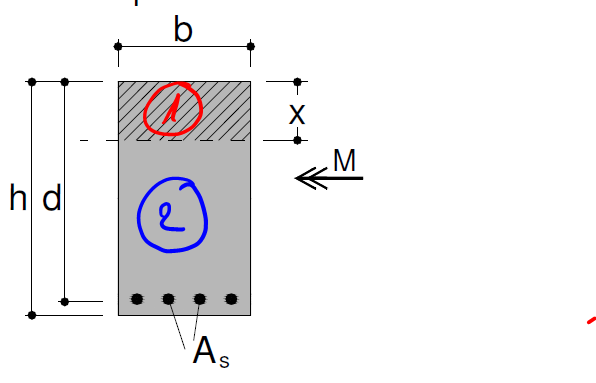
\includegraphics[width=0.6\linewidth]{images/Risse2QSRechtecko.PNG}




	
	\subsubsection{Rechteckquerschnitt mit Druckbewehrung}
	
	
	\begin{tabular}{p{0.4\linewidth}|p{0.4\linewidth}}
		
		Bemerkung		& Formel	 \\ \hline
		
		
		\hspace*{0pt} Spannungsberechnung	& $ E_{cm\infty} = \frac{E_{cm,0}}{1 + \varphi} $ und $ n = \frac{E_s}{E_{cm\infty}} $  \\
		
		Statisches Moment	& $ S_i = 0 = b \cdot x \cdot \frac{x}{2} + n \cdot A_s' (x - d') - (d - x) \cdot n \cdot A_s $  \\
		S$_i$ der ideellen Fläche muss bez. der neutralen Achse Null sein &	 \\
		
		Druckzonenhöhe		& $ x = n \cdot \frac{A_s + A_s'}{b} \left( \sqrt{1 + \frac{2 b d}{n} \frac{A_s + A_s' \frac{d'}{d}}{(A_s + A_s')^2} } - 1 \right) $   \\
		$ \rightarrow $ aus Bedigung S$_i$=0 &  \\
		
		Flächenmoment		& $ I_{Rechteck,i} = \frac{b \cdot x^3}{3} + n \cdot A_s' (x - d')^2 + n \cdot A_s (d - x)^2 $	  \\
		
		\hspace*{0pt} Verträglichkeitsbedingung & $ \frac{\varepsilon_s}{\varepsilon_c} = \frac{d - x}{x}
		\Rightarrow \varepsilon_s = \frac{d - x}{x} \varepsilon_c $	 \\
		& $ E_s \cdot \varepsilon_s = \sigma_s = E_s \cdot \varepsilon_c \frac{d - x}{x} = n \cdot \sigma_c \frac{d - x}{x} $		\\
		
		Stahlspannung			& $ \sigma_s = n \frac{M}{I_i} (d - x) $	 \\
		
	\end{tabular}


	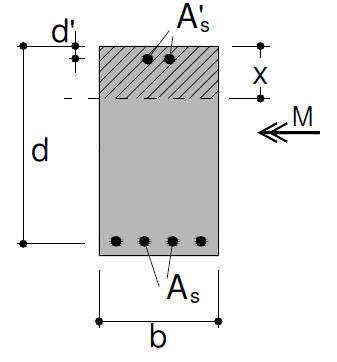
\includegraphics[width=0.4\linewidth]{images/Risse3QSRechteckm.PNG}





\subsubsection{Plattenbalkenquerschnitt}


	\begin{tabular}{p{0.4\linewidth}|p{0.6\linewidth}}
		
		Bemerkung		& Formel	 \\ \hline
		
		
		abklären ob x $ \leq $ h$_f$ oder x > h$_f$ & \\
		
		& $ S_i (x = h_f) =  b \cdot \frac{h_f^2}{2} + n \cdot A_s' (h_f - d') - n \cdot A_s (d - h_f)  $   \\
		\textcolor{red}{1} S$_i$ (x = h$_f$) > 0 $ \rightarrow $ Berechnen am Rechteck QS &	 \\
		\textcolor{red}{2} S$_i$ (x = h$_f$) < 0 $ \rightarrow $ Berechnen am Plattenbalken QS (Druck bis in Steg) &	 \\
		
		falls Plattenbalken: Statisches Moment	& $ S_i = 0 = (b - b_w) h_f \left( x - \frac{h_f}{2} \right) + \frac{b_w \cdot x^2}{2} + n \cdot A_s' (x - d') - n \cdot A_s (d - x) \rightarrow x $  \\
		
		Flächenmoment		& $ I_{i} = (b - b_w) \frac{h_f^3}{12} + (b - b_w) h_f \left( x - \frac{h_f}{2} \right)^2 + \frac{b_w \cdot x^3}{3} + n \cdot A_s' (x - d')^2 + n \cdot A_s (d - x)^2 $	  \\
		
		\hspace*{0pt} Verträglichkeitsbedingung & $ \frac{\varepsilon_s}{\varepsilon_c} = \frac{d - x}{x}
		\Rightarrow \varepsilon_s = \frac{d - x}{x} \varepsilon_c $	 \\
		& $ E_s \cdot \varepsilon_s = \sigma_s = E_s \cdot \varepsilon_c \frac{d - x}{x} = n \cdot \sigma_c \frac{d - x}{x} $		\\
		
		Stahlspannung			& $ \sigma_s = n \frac{M}{I_i} (d - x) $ \\
		
	\end{tabular}


	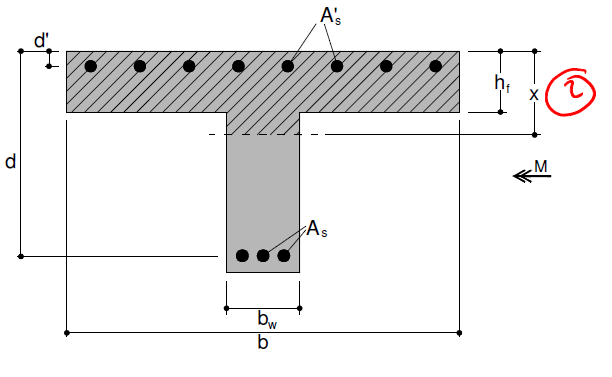
\includegraphics[width=0.5\linewidth]{images/Risse4Plattenbalken.PNG}

	
\end{multicols}

\end{landscape}